%! Author = sarge
%! Date = 2/10/2022

% Preamble
\documentclass[12pt]{article}
\author{Carlos Medina}
\title{PH 1110 Lab 4 CX17}

% Packages
\usepackage{amsmath}
\usepackage[margin=1in]{geometry}
\usepackage{graphicx, caption}
\usepackage{subcaption}
\usepackage{float}
\usepackage[separate-uncertainty=true, multi-part-units=repeat]{siunitx}
\usepackage{enumerate}
\usepackage[outputdir=../out]{minted}
\usepackage{titling}
\usepackage{textgreek}

\usemintedstyle{colorful}
\graphicspath{{../imgs/}}
\newcommand{\mps}[1]{\SI{#1}{\meter\per\second}}
\newcommand{\impls}[1]{\SI{#1}{\newton\second}}


% Document
\begin{document}
%    \posttitle{\par\end{center}}
    \setlength{\droptitle}{-60pt}
    \maketitle


    \section{Propagation of Uncertainty}
    \begin{enumerate}
        [1)]
        \item Python 3.6 code for propagation of uncertainty:
        \begin{minted}{python}
        ### 1: velocity
        v_Ai =0.3283 #initial velocity
        dv_Ai =0.01595 #uncertainty of velocity
        v_Af =0.2892 #final velocity
        dv_Af =0.0028 #uncertainty of "
        delta_vA =v_Af -v_Ai #change in velocity
        dvA =dv_Ai +dv_Af #propogation of uncertainty for velocity
        ### 2: mass
        m =0.4975 #measured mass of the cart in kg
        dm =0.0001 #uncertainty in "
        ### 3: momentum
        p_0 = (m *v_Ai) #initial momentum of the system
        dp_0 =p_0 * ((dm/m)+((dv_Ai)/abs(v_Ai))) #uncertainty in "
        #Some notes on the above equation
        #Don't need to do absolute value of m
        #because it's already positive
        p_f = (m *v_Af) #final momentum of the system
        #uncertainty in momentum
        dp_f =p_f * ((dm/m)+((dv_Af)/abs(v_Af)))
        delta_p =p_f -p_0 #change in momentum
        dp =dp_f +dp_0 #uncertainty of "
        print("change in momentum:",delta_p,"±",dp," kg * m/s")
        #print the change in momentum and its uncertainty

        #>> change in momentum: -0.019452249999999977 ± 0.009389874999999999  kg * m/s
        \end{minted}
    \end{enumerate}


    \section{Writing}
    \begin{enumerate}
        [1)]
        \item I made sure to not go too fast and to make sure everything was good
        \item ~
        %slow
        \begin{figure}[H]
            \begin{subfigure}[t]{0.5\textwidth}
                \centering
                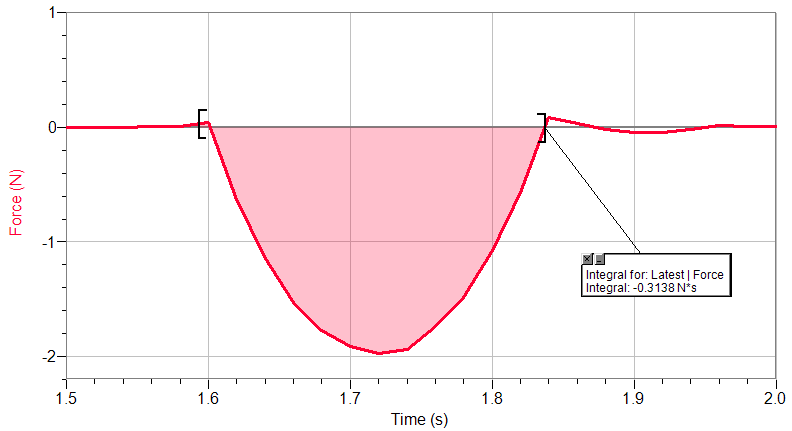
\includegraphics[width=3.2in]{slow_force}
                \caption{Slow force. The impulse measured is \impls{-0.3138}.}
            \end{subfigure}%
            ~
            \begin{subfigure}[t]{0.5\textwidth}
                \centering
                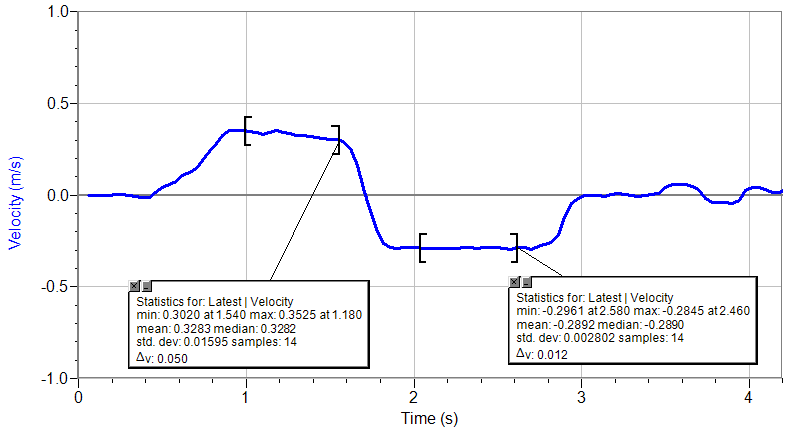
\includegraphics[width=3.2in]{slow_velo}
                \caption{Slow velocity. The initial velocity is \mps{0.3283} with \textsigma\ = \mps{0.0159}, and the final velocity is \mps{-.2890} with \textsigma\ = \mps{0.0028}}
            \end{subfigure}
            \caption{Slow trial measurements.}
        \end{figure}
        %slower
        \begin{figure}[H]
            \begin{subfigure}[t]{0.5\textwidth}
                \centering
                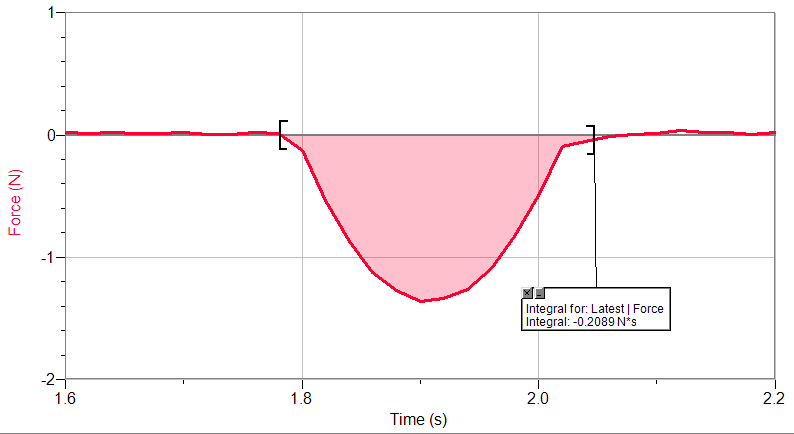
\includegraphics[width=3.2in]{slower_force}
                \caption{Slower force. The impulse measured is \impls{-0.2089}.}
            \end{subfigure}%
            ~
            \begin{subfigure}[t]{0.5\textwidth}
                \centering
                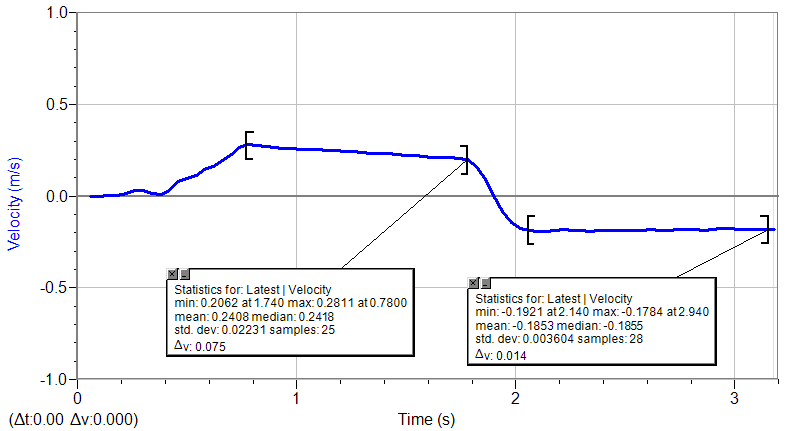
\includegraphics[width=3.2in]{slower_velo}
                \caption{Slower velocity. The initial velocity is \mps{0.2408} with \textsigma\ = \mps{0.0223}, and the final velocity is \mps{-.1853} with \textsigma\ = \mps{0.0004}}
            \end{subfigure}
            \caption{Slower trial measurements.}
        \end{figure}
        %slowest
        \begin{figure}[H]
            \begin{subfigure}[t]{0.5\textwidth}
                \centering
                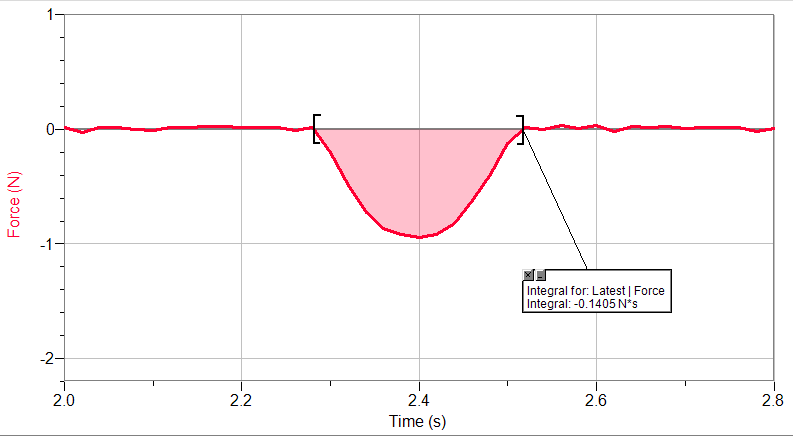
\includegraphics[width=3.2in]{slowest_force}
                \caption{Slowest force. The impulse measured is \impls{-0.1405}.}
            \end{subfigure}%
            ~
            \begin{subfigure}[t]{0.5\textwidth}
                \centering
                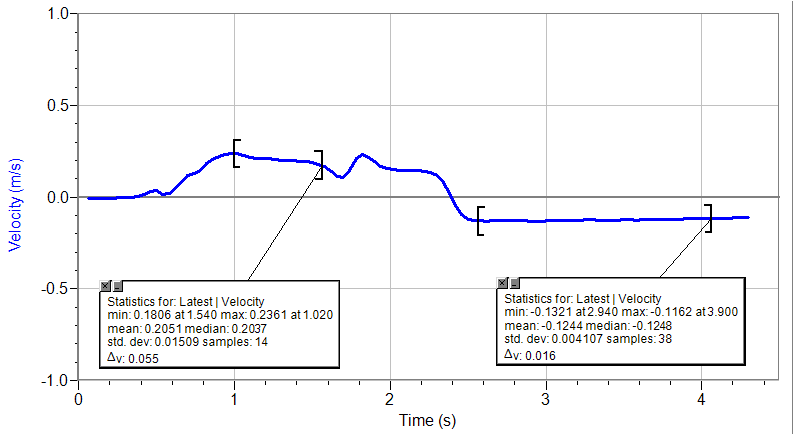
\includegraphics[width=3.2in]{slowest_velo}
                \caption{Slowest velocity. The initial velocity is \mps{0.2051} with \textsigma\ = \mps{0.0151}, and the final velocity is \mps{-.1244} with \textsigma\ = \mps{0.0041}}
            \end{subfigure}
            \caption{Slowest trial measurements.}
        \end{figure}
    \end{enumerate}
\end{document}